% arara: clean: {
% arara: --> extensions:
% arara: --> ['aux', 'bbl', 'bcf', 'blg', 'log', 'out', 'pdf', 'run.xml', 'toc']
% arara: --> }
% arara: lualatex: {
% arara: --> shell: yes,
% arara: --> draft: yes,
% arara: --> interaction: batchmode
% arara: --> }
% arara: biber
% arara: lualatex: {
% arara: --> shell: yes,
% arara: --> draft: no,
% arara: --> interaction: batchmode
% arara: --> }
% arara: lualatex: {
% arara: --> shell: yes,
% arara: --> draft: no,
% arara: --> interaction: batchmode
% arara: --> }
% arara: clean: {
% arara: --> extensions:
% arara: --> ['aux', 'bbl', 'bcf', 'blg', 'log', 'out', 'run.xml', 'toc']
% arara: --> }
\documentclass[
	12pt,
	oneside,
	appendixprefix=true
]{scrbook}
\usepackage[spanish]{babel}
\decimalpoint
\usepackage{diffcoeff}
\usepackage[intlimits]{mathtools}
\usepackage{amssymb}
\usepackage{amsthm}
\usepackage{graphicx}
\usepackage{minted}
\usepackage[
	citestyle=numeric,
	style=numeric,
	backend=biber,
]{biblatex}
\usepackage{hyperref}

\title{
	Una introducción acerca de los métodos de volúmenes finitos para
	una ecuación de transporte
}
\author{\scshape\name}
\date{\today}

% \addtokomafont{section}{\centering}
% \addtokomafont{subsection}{\centering}

\theoremstyle{definition}
\newtheorem{theorem}{Teorema}
\newtheorem{definition}{Definición}
\newtheorem{remark}{Observación}
\newtheorem{example}{Ejemplo}
\addbibresource{references.bib}

\providecommand{\name}{Carlos Aznarán} % Nombre
\renewcommand{\listingscaption}{Programa}
\renewcommand{\listoflistingscaption}{Lista de \listingscaption s}

\hypersetup{
	pdfencoding=auto,
	linktocpage=true,
	colorlinks=true,
	linkcolor=blue,
	urlcolor=magenta,
	pdfpagelabels,
	pdftex,
	pdfauthor={Carlos Aznarán Laos},
	pdftitle={Una introducción acerca de los métodos de volúmenes
			finitos para una ecuación de transporte},
	pdfsubject={Lecture},
	pdfkeywords={finite volume, pde, transport equation},
	pdfproducer={LuaHBTeX, Version 1.18.0 (TeX Live 2024/Arch Linux)},
	% bookmark=false
}

\clearpage
\pagestyle{empty}
\renewcommand*{\chapterpagestyle}{empty}


\begin{document}

\maketitle

\chapter*{Agradecimientos}

Con la conclusión de este trabajo, deseo expresar mi más sincero
agradecimiento a todas las personas que hicieron posible su
realización.

En primer lugar, a mi supervisor, Fidel Jara Huanca, profesor de la
Facultad de Ciencias de la Universidad Nacional de Ingeniería, por
brindarme la oportunidad de trabajar en este Taller de Investigación
vinculante a su proyecto del doctorado.
Le estoy profundamente agradecido por su invaluable apoyo durante los
últimos dos años, por su generosidad al compartir consejos, por la
motivación constante y, especialmente, por sus exhaustivas revisiones
y útiles sugerencias que enriquecieron enormemente este manuscrito.

Mi agradecimiento se extiende al matemático Jose Alcalde del
Instituto de Matemática y Ciencias Afines, por su colaboración y
trabajo conjunto tanto conmigo como con el profesor Jara.

De manera muy especial, quiero agradecer la estudiante de matemática
Karen Lizeth Silvera de la Universidad Nacional de San Antonio Abad
del Cusco.
A ella, que ha sido mi compañera en este camino, le doy gracias por
su apoyo incondicional y por ser un pilar fundamental durante todo
este proceso.

Finalmente, a mi familia y amigos, por su paciencia y aliento en cada
etapa de este reto.

\begin{frame}

	\begin{abstract}
		El método de los volúmenes finitos constituye una técnica
		numérica robusta para aproximar la solución de una ley de
		conservación
		\begin{math}
			\difcp{u}{t}+
			\difcp{f\left(u\right)}{x}=
			0
		\end{math},
		por funciones constantes por partes~\cite[p.~5]{Saeed2025}.
		Este enfoque se basa en discretizar el dominio computacional
		$\Omega\subset\mathbb{R}^{d}$ en una malla compuesta por celdas
		disjuntas
		\begin{math}
			\Omega^{h}=
			\bigcup_{j=1}^{N}
			\Omega_{j}
		\end{math},
		cuya unión cubre el dominio salvo un conjunto de medida nula.
		Para transformar el problema continuo en un sistema algebraico
		discreto, integre la EDP sobre cada celda $\Omega_{j}$.
		Las incógnitas del sistema son aproximaciones del valor medio de
		la solución en cada celda, lo que preserva localmente las
		propiedades de conservación de la EDP.

		\par\vskip\baselineskip\noindent
		{\textbf{Palabras clave}:
			Esquema de Alta Resolución,
			Limitador de flujo,
			Análisis de estabilidad,
			Variación total decreciente.}
		\par\vskip\baselineskip\noindent
		{\textbf{Clasificación Matemática por Temas}:
			35L04,
			35L65,
			35Q35,
			65L12,
			65M06,
			65M12.}
	\end{abstract}

	\pause

	\visible<.(1)>{
		\begin{figure}[ht!]
			\centering
			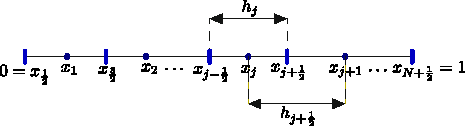
\includegraphics[width=.45\textwidth]{fv1d}
			\caption{
				Malla de volúmenes finitos 1D de $\Omega=\left(0,1\right)$.
				Los nodos de índices enteros
				\begin{math}
					{\big\{x_{j}\big\}}^{N}_{j=1}
				\end{math}
				representan los puntos de aproximación y los nodos de índices
				fraccionarios
				\begin{math}
					{\big\{x_{j+\tfrac{1}{2}}\big\}}^{N}_{j=1}
				\end{math}.
				\begin{math}
					x_{j}
				\end{math}
				es el centro de la celda
				\begin{math}
					\Omega_{j}=
					\big[
						x_{j-\tfrac{1}{2}},
						x_{j+\tfrac{1}{2}}
						\big]
				\end{math}
				cuyo tamaño es
				\begin{math}
					h_{j}=
					x_{j+\tfrac{1}{2}}-
					x_{j-\tfrac{1}{2}}
				\end{math}.
				La distancia entre dos celdas consecutivas es
				% \forall j=0,\dotsc,N:
				\begin{math}
					h_{j+\tfrac{1}{2}}=
					\frac{1}{2}\left(h_{j}+h_{j+1}\right)=
					x_{j+1}-x_{j}
				\end{math}.
			}
		\end{figure}
	}
\end{frame}

\tableofcontents

\part{Teoría}

\chapter{Sistema de leyes de conservación}

Presentamos un sistema de leyes de conservación en una dimensión
espacial, así como los ejemplos más destacados en la física de los
medios continuos.

\begin{definition}
	Sea $\Omega\subset\mathbb{R}^{p}$ un conjunto abierto.
	Un \textcolor{DarkBlue}{\bfseries sistema de leyes de conservación}
	\index{sistema de leyes de conservación} es
	\begin{equation}\label{eq:systemofconservationlaw}
		\diffp{\symbf{u}}{t}+
		\diffp{}{x}
		\symbf{f}\left(\symbf{u}\right)=
		\symbf{s}\left(\symbf{u},x\right).
	\end{equation}
	Donde $\Omega$ es el conjunto de estados,
	\begin{math}
		\symbf{f}\in\symbf{C}^{1}
		\left(\Omega,\mathbb{R}^{p}\right)
	\end{math}
	es la función flujo,
	\begin{math}
		\symbf{s}\in
		\symbf{C}^{1}
		\left(\Omega\times\mathbb{R},\mathbb{R}^{p}\right)
	\end{math}
	es la función fuente sin términos de derivadas de $\symbf{u}$ y
	\begin{math}
		\symbf{u}\in
		\symbf{C}^{1}
		\left(\mathbb{R}\times\left[0,\infty\right[,\Omega\right)
	\end{math} es la solución de~\eqref{eq:systemofconservationlaw}.
	\begin{align*}
		\symbf{f}\colon\Omega                                &
		\longrightarrow\mathbb{R}^{p}                        &
		\symbf{s}\colon\Omega\times\mathbb{R}                &
		\longrightarrow\mathbb{R}^{p}                        &
		\symbf{u}\colon\mathbb{R}\times\left[0,\infty\right[ &
		\longrightarrow\Omega                                  \\
		\begin{bmatrix}
			u_{1}  \\
			\vdots \\
			u_{p}
		\end{bmatrix}                                      &
		\longmapsto
		\begin{bmatrix}
			f_{1}  \\
			\vdots \\
			f_{p}
		\end{bmatrix},                                      &
		\left(\symbf{u},x\right)                             &
		\longmapsto
		\begin{bmatrix}
			s_{1}\left(\symbf{u},x\right) \\
			\vdots                        \\
			s_{p}\left(\symbf{u},x\right)
		\end{bmatrix},                     &
		\left(x,t\right)                                     &
		\longmapsto
		\begin{bmatrix}
			u_{1}\left(x,t\right) \\
			\vdots                \\
			u_{p}\left(x,t\right)
		\end{bmatrix}=
		\begin{bmatrix}
			u_{1}  \\
			\vdots \\
			u_{p}
		\end{bmatrix}.
	\end{align*}
\end{definition}
Si $I\subset\mathbb{R}$, entonces
de~\eqref{eq:systemofconservationlaw} se obtiene la ecuación de
balance que expresa que la variación en el tiempo de la cantidad
total en el medio es igual al flujo neto a través de la interface
más la contribución del término fuente.
\begin{equation*}
	\diff{}{t}
	\int_{I}\symbf{u}\dl x+
	{\symbf{f}\left(\symbf{u}\right)\Big|}_{\partial I}=
	\int_{I}\symbf{s}\left(\symbf{u},x\right)\dl x.
\end{equation*}

\begin{definition}
	Un sistema~\eqref{eq:systemofconservationlaw} es
	\textcolor{DarkBlue}{\bfseries hiperbólico}\index{hiperbólico} si y
	solo si
	\begin{equation}
		\forall\symbf{u}\in\Omega\!:
		\forall\omega\in\mathbb{R}\setminus\left\{0\right\}\!:
		\exists
		{\left\{
			\left(\lambda_{k},\symbf{r}_{k}\right)
			\right\}}^{p}_{k=1}\subset
		\mathbb{R}\times\mathbb{R}^{p}
		\text{ tal que }
		\symbf{A}\left(\symbf{u},\omega\right)
		\symbf{r}_{k}=
		\lambda_{k}
		\symbf{r}_{k}.
	\end{equation}
	Donde
	\begin{math}
		\symbf{A}\left(\symbf{u},\omega\right)\coloneqq
		\omega
		{
			\begin{bmatrix}
				\diffp{f_{i}}{u_{k}}
				\left(\symbf{u}\right)
			\end{bmatrix}}_{\substack{1\leq i\leq p\\1\leq k\leq p}}
	\end{math}
	es un múltiplo de la matriz jacobiana de $\mathbf{f}$.
\end{definition}

\begin{definition}
	Un \textcolor{DarkBlue}{\bfseries problema de Riemann}
	\index{problema de Riemann} es un problema de valor inicial
	asociado a~\eqref{eq:systemofconservationlaw}
	\begin{equation}\label{eq:cauchysystemofconservationlaw}
		\begin{cases}
			\diffp{\symbf{u}}{t}+
			\diffp{}{x}
			\symbf{f}\left(\symbf{u}\right)=
			\symbf{s}\left(\symbf{u},x\right) &
			\text{en }\mathbb{R}\times\left(0,\infty\right). \\
			\symbf{u}=\symbf{u}_{0}           &
			\text{en }\mathbb{R}\times\left\{t=0\right\}.
		\end{cases}
	\end{equation}
	Donde $\symbf{u}_{l},\symbf{u}_{r}\in\Omega$ son los estados y
	\begin{equation*}
		\symbf{u}_{0}\left(x\right)=
		\begin{cases}
			\symbf{u}_{l}, & x<0. \\
			\symbf{u}_{r}, & x>0.
		\end{cases}
	\end{equation*}
\end{definition}

\begin{definition}
	El problema de valor inicial y de frontera asociado
	a~\eqref{eq:systemofconservationlaw} es
	\begin{equation}
		\begin{dcases}
			\diffp{\symbf{u}}{t}+
			\diffp{}{x}\symbf{f}\left(\symbf{u}\right)=
			\symbf{s}\left(\symbf{u},x\right) &
			\text{ en }I\times\left(0,T\right].         \\
			\symbf{u}=\symbf{u}_{0}           &
			\text{c.t.p. en }I\times\left\{t=0\right\}. \\
			\symbf{u}=\symbf{g}               &
			\text{ en }\partial I\times\left[0,T\right].
		\end{dcases}
	\end{equation}
\end{definition}

\begin{example}[La ecuación de Bateman-Burgers no viscosa]\index{ecuación de Burgers}
	\begin{equation}
		\begin{dcases}
			\diffp{u}{t}+
			\frac{1}{2}\diffp{u^{2}}{x}=0 &
			\text{ en }I\times\left(0,T\right].         \\
			u=u_{0}                       &
			\text{c.t.p. en }I\times\left\{t=0\right\}. \\
			u=g                           &
			\text{ en }\partial I\times\left[0,T\right].
		\end{dcases}
	\end{equation}
	% \begin{equation*}
	% 	\diffp{u}{t}+
	% 	u\diffp{u}{x}-
	% 	\nu\diffp[2]{u}{x}=
	% 	0.
	% \end{equation*}
\end{example}

\begin{example}%[Ecuación de Buckley-Leverett]
	La ecuación clásica de
	Buckley-Leverett\index{ecuación de Buckley-Leverett}
	es un modelo simple para un flujo de fluido de dos fases en un medio
	poroso.
	Una aplicación es la recuperación secundaria mediante impulsión de
	agua en la simulación de yacimientos de petróleo.
	\begin{equation}
		\begin{dcases}
			\diffp{u}{t}+
			\diffp{}{x}
			f\left(u\right)=0 &
			\text{ en }I\times\left(0,T\right].         \\
			u=u_{0}                       &
			\text{c.t.p. en }I\times\left\{t=0\right\}. \\
			u=g                           &
			\text{ en }\partial I\times\left[0,T\right].
		\end{dcases}
	\end{equation}
	\begin{equation*}
		f\left(s\right)=
		\frac{\frac{\kappa_{\text{rel,water}}\left(s\right)}{\mu_{\text{water}}}}{
			\frac{\kappa_{\text{rel,water}}\left(s\right)}{\mu_{\text{water}}}+
			\frac{\kappa_{\text{rel,oil}}\left(s\right)}{\mu_{\text{oil}}}
		}.
	\end{equation*}
\end{example}

\begin{example}[$p$-sistema]\index{$p$-sistema}
	\begin{equation*}
		\begin{cases}
			\diffp{v}{t}-\diffp{u}{x}=0               &
			\text{en }\mathbb{R}\times\left(0,\infty\right). \\
			\diffp{u}{t}+\diffp{}{x}p\left(v\right)=0 &
			\text{en }\mathbb{R}\times\left(0,\infty\right).
		\end{cases}
	\end{equation*}
\end{example}


% Sistema de fluidos % de la dinámica de gases
\begin{example}[Ecuaciones de Euler]\index{ecuaciones de Euler}
	\begin{equation*}
		\begin{dcases}
			\diffp{\rho}{t}+
			\sum_{j=1}^{3}
			\diffp{}{x_{j}}
			\left(\rho u_{j}\right)=0                   &
			\text{en }\mathbb{R}\times\left(0,\infty\right). \\
			\forall i\in\left\{1,2,3\right\}:
			\diffp{}{t}
			\left(\rho u_{i}\right)+
			\sum_{j=1}^{3}
			\diffp{}{x_{j}}
			\left(\rho u_{i}u_{j}+p\delta_{ij}\right)=0 &
			\text{en }\mathbb{R}\times\left(0,\infty\right). \\
			\diffp{}{t}
			\left(\rho e\right)+
			\sum_{j=1}^{3}
			\diffp{}{x_{j}}
			\left(\left(\rho e+p\right)u_{j}\right)=0   &
			\text{en }\mathbb{R}\times\left(0,\infty\right).
		\end{dcases}
	\end{equation*}
\end{example}

\chapter{Esquemas de volúmenes finitos}

Considere el problema de Cauchy~\eqref{eq:cauchysystemofconservationlaw}
donde~\eqref{eq:systemofconservationlaw} es hiperbólico.
Consideremos $C_{j}=\left[x_{j-\frac{1}{2}},x_{j+\frac{1}{2}}\right]\subset\mathbb{R}$
\begin{equation*}
	\symbf{v}^{n}_{j}\approx
	\frac{1}{\left|C_{j}\right|}
	\int_{C_{j}}
	\symbf{u}\left(x,t_{n}\right)\dl{\symbf{x}}.
\end{equation*}
\begin{equation*}
	\diff{}{t}
	\int_{C_{j}}
	\symbf{u}\left(x,t\right)\dl x+
	f\left(u\left(x_{j+\frac{1}{2}},t\right)\right)-
	f\left(u\left(x_{j-\frac{1}{2}},t\right)\right)=
	\symbf{0}.
\end{equation*}
\begin{equation*}
	\symbf{v}^{n+1}_{j}=
	\symbf{H}\left(\symbf{v}^{n}_{j-k},\dotsc,\symbf{v}^{n}_{j+k}\right).
\end{equation*}

\section{Método de Godunov}

\begin{equation*}
	\symbf{w}\left(x,t\right)=
	\symbf{w}_{R}
	\left(\frac{x}{t};\symbf{u}_{L},\symbf{u}_{R}\right)
\end{equation*}

\section{Método de Roe}

\section{Método de Rusanov}

% clawpack, fipy
\part{Aplicaciones}
\chapter{Implementación de las técnicas}

A continuación, pensamos dos estrategias para tentar resolver por el
método de los volúmenes finitos de un
\textcolor{DarkRed}{sistema EDP complicado}.
Se trata de resolver un sistema EDP a la vez, de menor a mayor
dificultad.
Suponga que $\Omega\subset\mathbb{R}^{3}$ es un conjunto abierto y
$\symbf{a},\symbf{b}\in\mathbb{R}^{3}\setminus\left\{\symbf{0}\right\}$.

\section{Primera estrategia}

\begin{equation*}
	\eqref{eq:advectionsystem}\implies
	\eqref{eq:advectionreactionsystem}\implies
	\eqref{eq:advectionreactionsystemquaslinearnonhomogeneous}\implies
	\mathcolor{DarkRed}{\eqref{eq:complicatedsystem}}.
\end{equation*}

\section{Segunda estrategia}

\begin{equation*}
	\eqref{eq:advectionsystem}\implies
	\eqref{eq:advectionreactionsystemquaslinear}\implies
	\eqref{eq:advectionreactionsystemquaslinearnonhomogeneous}\implies
	\mathcolor{DarkRed}{\eqref{eq:complicatedsystem}}.
\end{equation*}

\subsection*{Sistema EDP de advección lineal homogéneo}

Encuentre
\begin{math}
	\symbf{u}\in
	\symbf{C}^{1}\left(I\times\left[0,T\right],\Omega\right)
\end{math}
en el problema de valor inicial y de frontera~\eqref{eq:advectionsystem}
\begin{equation}\label{eq:advectionsystem}
	\begin{cases}
		\diffp{\symbf{u}}{t}+\diffp{}{x}\symbf{f}\left(\symbf{u}\right)=
		\symbf{0}     &
		\text{ en }I\times\left(0,T\right].   \\
		\symbf{u}                                                      =
		\symbf{u}_{0} &
		\text{ en }I\times\left\{t=0\right\}. \\
		\symbf{u}                                                      =
		\symbf{0}     &
		\text{ en }\partial I\times\left[0,T\right].
	\end{cases}
\end{equation}
Donde
\begin{math}
	\symbf{u}_{0}\in
	{\symbf{L}^{\infty}_{\text{loc}}\left(I\right)}^{3}
\end{math}
es conocida y
\begin{math}
	\symbf{f}\in
	\symbf{C}^{1}\left(\Omega,\mathbb{R}^{3}\right)
\end{math}
es dada por
\begin{math}
	\symbf{f}\left(\symbf{u}\right)=
	\symbf{a}\odot\symbf{u}
\end{math}.

\subsection*{Sistema EDP de advección reacción lineal}

Encuentre
\begin{math}
	\symbf{u}\in
	\symbf{C}^{1}\left(I\times\left[0,T\right],\Omega\right)
\end{math}
en el problema de valor inicial y de frontera~\eqref{eq:advectionreactionsystem}
\begin{equation}\label{eq:advectionreactionsystem}
	\begin{cases}
		\diffp{\symbf{u}}{t}+
		\diffp{}{x}\symbf{f}\left(\symbf{u}\right)               =
		\symbf{s}\left(\symbf{u}\right) &
		\text{ en }I\times\left(0,T\right].   \\
		\symbf{u}                                                                     =
		\symbf{u}_{0}                   &
		\text{ en }I\times\left\{t=0\right\}. \\
		\symbf{u}                                                                     =
		\symbf{0}                       &
		\text{ en }\partial I\times\left[0,T\right].
	\end{cases}
\end{equation}
Donde
\begin{math}
	\symbf{u}_{0}\in
	{\symbf{L}^{\infty}_{\text{loc}}\left(I\right)}^{3}
\end{math},
\begin{math}
	\symbf{s}\colon\Omega\to
	\mathbb{R}^{3}
\end{math}
son conocidas y
\begin{math}
	\symbf{f}\in
	\symbf{C}^{1}\left(\Omega,\mathbb{R}^{3}\right)
\end{math}
es dada por
\begin{math}
	\symbf{f}\left(\symbf{u}\right)=
	\symbf{a}\odot\symbf{u}
\end{math},
\begin{math}
	\symbf{s}\left(\symbf{u}\right)=
	\symbf{b}\odot\symbf{u}
\end{math}.

\subsection*{Sistema EDP de advección reacción cuasilineal I}

Encuentre
\begin{math}
	\symbf{u}\in
	\symbf{C}^{1}\left(I\times\left[0,T\right],\Omega\right)
\end{math}
en el problema de valor inicial y de frontera~\eqref{eq:advectionreactionsystemquaslinear}
\begin{equation}\label{eq:advectionreactionsystemquaslinear}
	\begin{cases}
		\diffp{\symbf{u}}{t}+\diffp{}{x}\symbf{f}\left(\symbf{u}\right)=
		\symbf{s}\left(\symbf{u}\right) & \text{ en }I\times\left(0,T\right].          \\
		\symbf{u}                                                      =
		\symbf{u}_{0}                   & \text{ en }I\times\left\{t=0\right\}.        \\
		\symbf{u}                                                      =
		\symbf{0}                       & \text{ en }\partial I\times\left[0,T\right].
	\end{cases}
\end{equation}
Donde
\begin{math}
	\symbf{u}_{0}\in
	{\symbf{L}^{\infty}_{\text{loc}}\left(I\right)}^{3}
\end{math},
\begin{math}
	\symbf{s}\colon\Omega\to
	\mathbb{R}^{3}
\end{math}
son conocidas y
\begin{math}
	\symbf{f}\in
	\symbf{C}^{1}\left(\Omega,\mathbb{R}^{3}\right)
\end{math}
es dada por
\begin{math}
	\symbf{f}\left(\symbf{u}\right)=
	\symbf{a}\odot\symbf{u}+
	\mathcolor{DarkRed}{a_{1}u_{1}\left(u_{2}-1\right)\symbf{e_{1}}}
\end{math},
\begin{math}
	\symbf{s}\left(\symbf{u}\right)=
	\symbf{b}\odot\symbf{u}
\end{math}.
% -\int^{x}\symbf{b}\odot\symbf{u}\dl y

\subsection*{Sistema EDP de advección reacción cuasilineal II}

Encuentre
\begin{math}
	\symbf{u}\in
	\symbf{C}^{1}\left(I\times\left[0,T\right],\Omega\right)
\end{math}
en el problema de valor inicial y de frontera~\eqref{eq:advectionreactionsystemquaslinearnonhomogeneous}
\begin{equation}\label{eq:advectionreactionsystemquaslinearnonhomogeneous}
	\begin{cases}
		\diffp{\symbf{u}}{t}+\diffp{}{x}\symbf{f}\left(\symbf{u}\right)=
		\symbf{s}\left(\symbf{u}\right) & \text{ en }I\times\left(0,T\right].          \\
		\symbf{u}                                                      =
		\symbf{u}_{0}                   & \text{ en }I\times\left\{t=0\right\}.        \\
		\symbf{u}                                                       =
		\symbf{0}                       & \text{ en }\partial I\times\left[0,T\right].
	\end{cases}
\end{equation}
Donde
\begin{math}
	\symbf{u}_{0}\in
	{\symbf{L}^{\infty}_{\text{loc}}\left(I\right)}^{3}
\end{math},
\begin{math}
	\symbf{s}\colon\Omega\to
	\mathbb{R}^{3}
\end{math}
son conocidas y
\begin{math}
	\symbf{f}\in
	\symbf{C}^{1}\left(\Omega,\mathbb{R}^{3}\right)
\end{math}
es dada por
\begin{math}
	\symbf{f}\left(\symbf{u}\right)=
	\symbf{a}\odot\symbf{u}+
	\mathcolor{DarkRed}{a_{1}u_{1}\left(u_{2}-1\right)\symbf{e_{1}}}
\end{math},
\begin{math}
	\symbf{s}\left(\symbf{u}\right)=
	u_{2}u_{3}\symbf{b}
	% \begin{bmatrix}
	% 	b_{1}u_{2}u_{3}  \\
	% 	-b_{2}u_{2}u_{3} \\
	% 	-b_{3}u_{2}u_{3}
	% \end{bmatrix}
\end{math}.

\subsection*{Sistema EDP de advección reacción cuasilineal III}

Encuentre
\begin{math}
	\symbf{u}\in
	\symbf{C}^{1}\left(I\times\left[0,T\right],\Omega\right)
\end{math}
en el problema de valor inicial y de frontera~\eqref{eq:advectionreactionsystemquaslinearnonhomogeneous}
\begin{equation}\label{eq:advectionreactionsystemquaslinearnonhomogeneous}
	\begin{cases}
		\diffp{\symbf{u}}{t}+\diffp{}{x}\symbf{f}\left(\symbf{u}\right)=
		\symbf{s}\left(\symbf{u}\right) & \text{ en }I\times\left(0,T\right].          \\
		\symbf{u}                                                      =
		\symbf{u}_{0}                   & \text{ en }I\times\left\{t=0\right\}.        \\
		\symbf{u}                                                       =
		\symbf{0}                       & \text{ en }\partial I\times\left[0,T\right].
	\end{cases}
\end{equation}
Donde
\begin{math}
	\symbf{u}_{0}\in
	{\symbf{L}^{\infty}_{\text{loc}}\left(I\right)}^{3}
\end{math},
\begin{math}
	\symbf{s}\colon\Omega\to
	\mathbb{R}^{3}
\end{math}
son conocidas y
\begin{math}
	\symbf{f}\in
	\symbf{C}^{1}\left(\Omega,\mathbb{R}^{3}\right)
\end{math}
es dada por
\begin{math}
	\symbf{f}\left(\symbf{u}\right)=
	\symbf{a}\odot\symbf{u}+
	\mathcolor{DarkRed}{a_{1}u_{1}\left(u_{2}-1\right)\symbf{e_{1}}}
\end{math},
\begin{math}
	\symbf{s}\left(\symbf{u}\right)=
	u_{2}u_{3}\symbf{b}-\beta u_{1}\symbf{e}_{1}
	% \begin{bmatrix}
	% 	b_{1}u_{2}u_{3}-\beta u_{1} \\
	% 	-b_{2}u_{2}u_{3}            \\
	% 	-b_{3}u_{2}u_{3}
	% \end{bmatrix}
\end{math}.

\subsection*{\color{DarkRed}Sistema EDP complicado}

Encuentre
\begin{math}
	\symbf{u}\in
	\symbf{C}^{1}\left(I\times\left[0,T\right],\Omega\right)
\end{math}
en el problema de valor inicial y de frontera~\eqref{eq:complicatedsystem}
\begin{equation}\label{eq:complicatedsystem}
	\begin{cases}
		\diffp{\symbf{u}}{t}+\diffp{}{x}\symbf{f}\left(\symbf{u}\right)=
		\symbf{s}\left(\symbf{u}\right) & \text{ en }I\times\left(0,T\right].          \\
		\symbf{u}                                                      =
		\symbf{u}_{0}                   & \text{ en }I\times\left\{t=0\right\}.        \\
		\symbf{u}                                                       =
		\symbf{0}                       & \text{ en }\partial I\times\left[0,T\right].
	\end{cases}
\end{equation}
Donde
\begin{math}
	\symbf{u}_{0}\colon I\to
	\mathbb{R}^{3}
\end{math},
\begin{math}
	\symbf{s}\colon\Omega\to
	\mathbb{R}^{3}
\end{math}
son conocidas y
\begin{math}
	\symbf{f}\colon\Omega\to
	\mathbb{R}^{3}
\end{math}
es dada por
\begin{math}
	\symbf{f}\left(\symbf{u}\right)=
	\symbf{a}\odot\symbf{u}+
	\mathcolor{DarkRed}{a_{1}u_{1}\left(u_{3}-1\right)\symbf{e_{1}}}
\end{math},
\begin{math}
	\symbf{s}\left(\symbf{u}\right)=
	u_{2}u_{3}\Phi\symbf{b}-\beta u_{1}\symbf{e}_{1}
	% \begin{bmatrix}
	% 	b_{1}u_{2}u_{3}\Phi-\beta u_{1} \\
	% 	-b_{2}u_{2}u_{3}\Phi            \\
	% 	-b_{3}u_{2}u_{3}\Phi
	% \end{bmatrix}
\end{math}.

\chapter{Resultados}

%https://mladenivkovic.github.io/work.html
% \begin{figure}[ht!]
% 	\centering
% 	\includegraphics[width=.8\paperwidth]{1}
% 	\includegraphics[width=.8\paperwidth]{2}
% 	\includegraphics[width=.8\paperwidth]{3}
% \end{figure}



\appendix

\chapter{Símbolos}

% https://ntrs.nasa.gov/api/citations/19880008959/downloads/19880008959.pdf
El producto de Hadamard se define como
\begin{align*}
	\odot\colon\mathbb{R}^{n}\times\mathbb{R}^{n} & \longrightarrow\mathbb{R}^{n} \\
	\left(
	\begin{bmatrix}
			a_{1}  \\
			\vdots \\
			a_{n}
		\end{bmatrix},
	\begin{bmatrix}
			b_{1}  \\
			\vdots \\
			b_{n}
		\end{bmatrix}
	\right)                                       & \longmapsto
	\begin{bmatrix}
		a_{1}b_{1} \\
		\vdots     \\
		a_{n}b_{n}
	\end{bmatrix}.
\end{align*}
El producto exterior se define como
\begin{align*}
	\otimes\colon\mathbb{R}^{m}\times\mathbb{R}^{n} & \longrightarrow\mathbb{R}^{m\times n} \\
	\left(
	\begin{bmatrix}
			a_{1}  \\
			\vdots \\
			a_{m}
		\end{bmatrix},
	\begin{bmatrix}
			b_{1}  \\
			\vdots \\
			b_{n}
		\end{bmatrix}
	\right)                                         & \longmapsto
	\begin{bmatrix}
		a_{1}b_{1} & \cdots & a_{1}b_{n} \\
		\vdots     & \ddots & \vdots     \\
		a_{m}b_{1} & \cdots & a_{m}b_{n}
	\end{bmatrix}.
\end{align*}
\nocite{*}
\printbibliography[title={Referencias},heading=bibintoc]

\end{document}
